\chapter{The Large Hadron Collider}

\section{Introduction}
The Large Hadron Collider (LHC) is a 26.7 kilometer-long, two-ring particle accelerator and collider located on the border of France and Switzerland at the European Organization for Nuclear Research (CERN).  During normal operations the LHC maintains two counter-rotating beams of proton bunches that collide at four interaction points (IP) with up to $\sqrt{s}=14$ TeV center of mass energy and a luminosity of 10$^{34}$cm$^{-2}$s$^{-1}$.  The ALICE (Point 2), ATLAS (Point 1), CMS (Point 5), and LHC-b experiments each have a detector at one of these interaction points as scene in Figure \ref{fig:lhcips} .  The CMS and ATLAS are general-purpose detectors while LHC-b specializes in beauty quark studies.  ALICE is a heavy-ion experiment which uses $^{208}Pb-p$ or $^{208}Pb-^{208}Pb$ collisions that can also be produced by the LHC.

\begin{figure}[h]
	\centering
	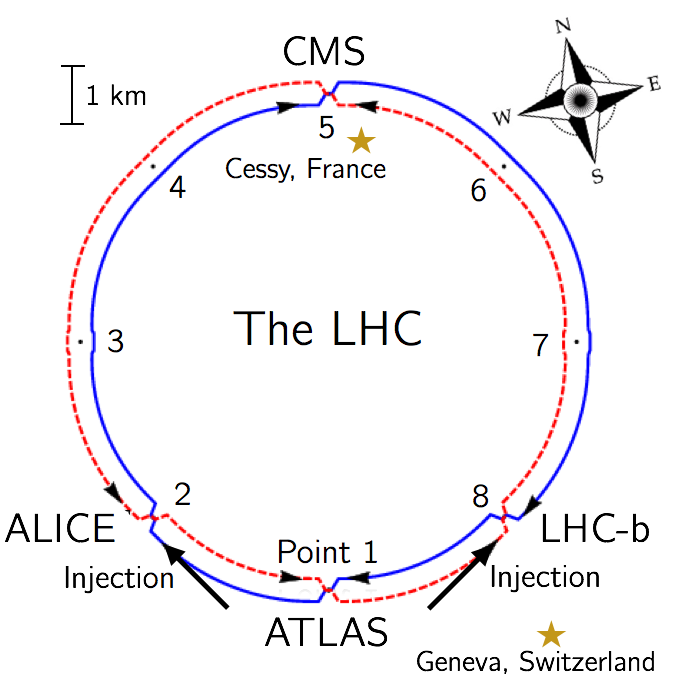
\includegraphics[width=0.7\linewidth]{Figures/LHC_IPs}
	\caption[LHC interaction points]{Interaction points of the LHC}
	\label{fig:lhcips}
\end{figure}


\section{Injection Complex}
In order to bring the protons from rest up to their target collision energy a series of accelerators, as shown in Figure \ref{fig:lhcsketch}, are used.  The acceleration sequence begins with the injection of hydrogen gas into a duoplasmatron.  Here a bombardment of electrons ionize the hydrogen atoms while an electric field pushes them through the duoplasmatron cavity. The result is 100 keV protons being passed on to a quadrapole magnet which guides them into the aperture of a linear accelerator (LINAC2).  The radio frequency (RF) cavities in LINAC2 accelerate the protons up to 50 MeV.  At this point the protons are sent into one of four rings in the Proton Synchrotron Booster (PSB).  The PSB repeatedly accelerates the protons around a circular path until they reach an energy of 1.4 GeV.  The bunches of protons from each PSB ring are then sequentially injected into the single-ringed Proton Synchrotron (PS).  Each bunch injected into the PS are captured by one of the "buckets" (Figure \ref{fig:rfbucket}) provided by the PS RF system which also manipulates the bunches into the desired profile and proton density. These proton bunches are accelerated to 25 GeV and injected into the Super Proton Synchrotron (SPS) where they are accelerated to 450 GeV.  Finally the proton bunches are injected into the LHC ring where they are accelerated to 6.5 TeV and collided in 25 ns intervals to yield a center of mass energy of $\sqrt{s} = 13$ TeV.

\begin{figure}[h]
	\centering
	\includegraphics[width=1.0\linewidth]{Figures/LHC_sketch1}
	\caption{Layout of LHC accelerator complex \cite{Evans_2008}.}
	\label{fig:lhcsketch}
\end{figure}

\begin{figure}[h]
	\centering
	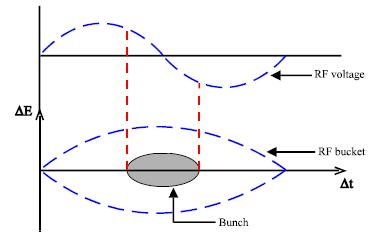
\includegraphics[width=0.7\linewidth]{Figures/RFbucket}
	\caption{Proton bunch capture onto RF bucket \cite{Baird:1017689}.}
	\label{fig:rfbucket}
\end{figure}


\section{Tunnel and Magnets}
The LHC was designed to produce collisions with up to $\sqrt{s} = 14$ TeV.  That requires confining and guiding 7 TeV protons around the circumference of the LHC ring.  The ring is housed in a 4 meter-wide underground tunnel that ranges in depth between 45 and 170 meters below the surface.  This tunnel was repurposed from the Large Electron-Positron (LEP) Collider which previously occupied the space.  For this reason the tunnel is not completely circular but is instead made up of alternating curved and straight sections of 2500 m and 530 m in length respectively.  The straight sections, labeled 1-8 in Figure \ref{fig:lhcips}, are used as either experimental facilities or sites for hardware necessary for LHC operations such as RF cavities for momentum cleaning, quadrupole magnets for beam focusing, and sextupole magnets for acceleration and betatron cleaning. 

Steering a 7 TeV proton beam around the curved sections requires a magnetic field of 8.33 Tesla which is provided by 1223 superconducting dipole magnets cooled to 1.9 K.  A cross section of the LHC dipole is shown in Figure \ref{fig:lhcdipole}.  Supercooled liquid helium flows through the heat exchanger pipe to cool the iron yolk to a temperature of 1.9 K.  Ultra high vacuum is maintainted in the outer volume to provide a layer of thermal insulation between the inner volume and the outer steel casing.  Inside the iron yolk is a twin bore assembly of niobium-titanium superconducting coils.  Two parallel beam pipes are located within the focus of the superconducting coils.  This is the ultra high vacuum region where the subatomic particles are confined as they travel around the LHC ring.

\begin{figure}[h]
	\centering
	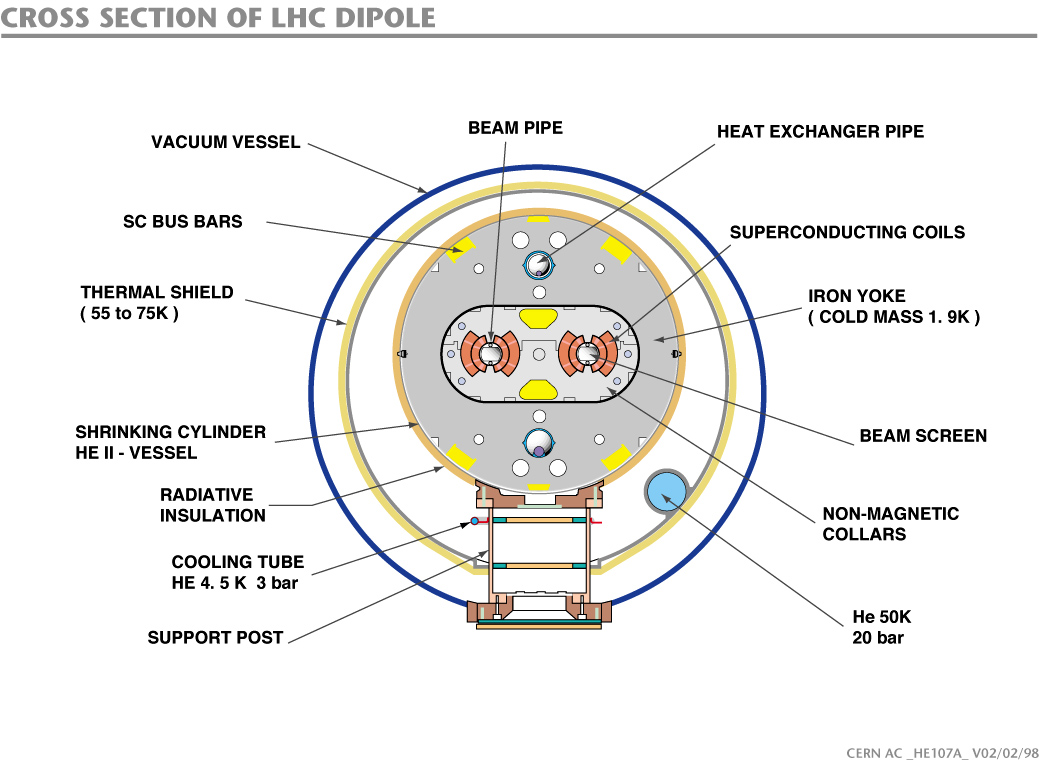
\includegraphics[width=0.7\linewidth]{Figures/LHCdipole}
	\caption{Cross section of LHC dipole \cite{dipole} }
	\label{fig:lhcdipole}
\end{figure}


\section{Luminosity} 
The number of events generated per second for specific process having cross-section $\sigma_{event}$ is given by:
\begin{equation}
\frac{dN_{event}}{dt} = L\sigma_{event}
\end{equation}
where $L$ in the machine luminosity.  The machine luminosity for a Gaussian beam distribution can be written in terms of the beam parameters as:
\begin{equation}
L = \frac{N^{2}_{b}n_{b}f_{rev}\gamma_{r}}{4\pi\epsilon_{n}\beta*}F
\end{equation}
where $N_{b}$ is particle density in each bunch, $n_{b}$ is the number of bunches in each beam, $f_{rev}$ is the frequency of revolution, and $\gamma_{r}$ is the relativistic gamma factor.  The variables $\epsilon_{n}$ and $\beta*$ are the normalized transverse beam emittance and the beta function at the IP respectively, while $F$ is the geometric reduction factor depending due to the beams' crossing angle at the IP. \cite{Evans_2008}

The total number of events produced over a given amount of time would then be
\begin{equation}
N_{event} = \sigma_{event}\int Ldt = \sigma_{event}L_{integrated}.
\end{equation}
The integrated luminosity delivered each year to the CMS experiment is shown in \ref{fig:intlumirun2}.  The analysis presented here uses data collected from the 2016, 2017, and 2018 campaigns which gives a combined integrated luminosity of 158.7 fb$^{-1}$.
\begin{figure}[h]
	\centering
	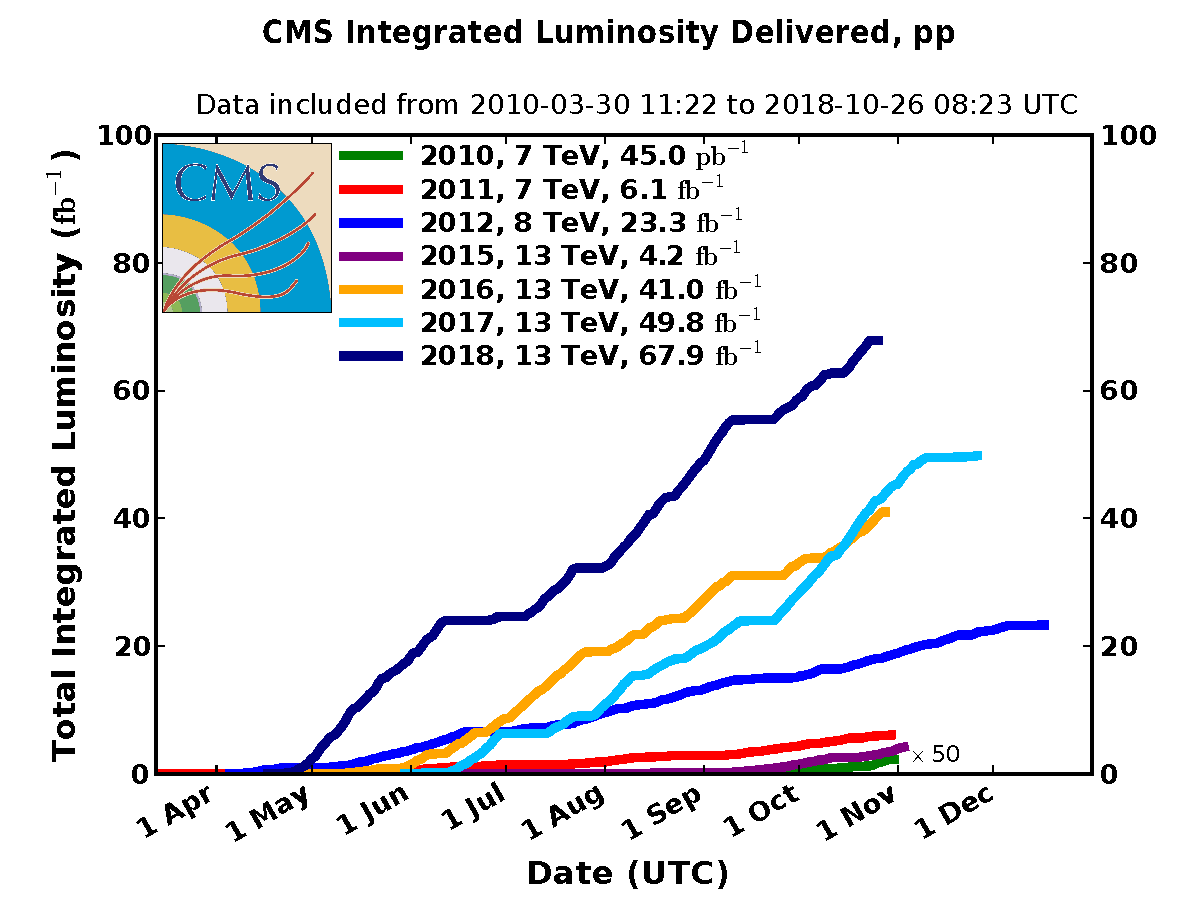
\includegraphics[width=0.7\linewidth]{Figures/Int_lumi_run2}
	\caption{Integrated luminosity delivered by the LHC to the CMS experiment each year from 2010-2018.}
	\label{fig:intlumirun2}
\end{figure}



